\chapter{PROCEDURES}
\thumbtab{Procedures}{0}
\minitoc
\cleardoublepage

\newgeometry{
    inner = 10mm,
    outer = 50mm,
    bottom=8mm,
    top=12mm,
}

\section{START-UP}

\subsection{PRE-START}
\begin{checklistenumerate}
    \blueitem{\hyperref[fig:proc:prestart:flcscheck]{FLCS Check}}{
    \marginpar{%
        \centering
        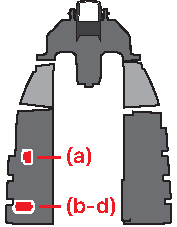
\includegraphics[
            width = \cockpitfigwidth,
        ]{F16_proc_start-up_flcs-check_v01.pdf}
        % \captionof*{figure}{\textbf{1. FLCS Check}}
        \captionof{figure}{\blue{FLCS Check}}
        \label{fig:proc:prestart:flcscheck}
    }
    \begin{subenumerate}
        \item \textbf{Main PWR Switch}\cbstart \dotfill \textbf{BATT}\cbend
        \begin{itemize}
            \item \textbf{FLCS RLY Light} -- \textbf{ON}
        \end{itemize}
        \item \textbf{FLCS PWR TEST} \dotfill \textbf{TEST (hold)}
        \item \textbf{Test Lights} \dotfill \textbf{Verify}
        \begin{itemize}
            \item \textbf{ACFT BATT TO FLCS} -- \textbf{ON}
            \item \textbf{FLCS PMG} -- \textbf{ON}
            \item \textbf{FLCS PWR} -- \textbf{ON}
            \item \textbf{FLCS RLY} -- \textbf{OFF}
        \end{itemize}
        \item \textbf{FLCS PWR TEST} \dotfill \textbf{Release}
    \end{subenumerate}}
    \blueitem{\hyperref[fig:proc:prestart:mainpower]{Main Power}}{
    \marginpar{%
        \centering
        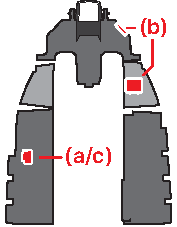
\includegraphics[
            width = \cockpitfigwidth,
        ]{F16_proc_start-up_main-power_v01.pdf}
        \captionof{figure}{\blue{Main Power}}
        \label{fig:proc:prestart:mainpower}
    }
    \begin{subenumerate}
        \item \textbf{Main PWR Switch}\cbstart \dotfill \textbf{MAIN}\cbend
        \item \textbf{Warning Lights} \dotfill \textbf{Check}
        \begin{itemize}
            \item \textbf{ELEC SYS} -- \textbf{ON}
            \item \textbf{HYD/OIL PRESS} -- \textbf{ON}
            \item \textbf{FLCS RLY} -- \textbf{ON}
            \item \textbf{SEC} -- \textbf{ON}
            \item \textbf{ENGINE} -- \textbf{ON}
        \end{itemize}
        \item \textbf{EPU Lights} \dotfill \textbf{Confirm OFF}
        \begin{itemize}
            \item \textbf{EPU GEN Light} -- \textbf{OFF}
            \item \textbf{EPU PMG Light} -- \textbf{OFF}
        \end{itemize}
    \end{subenumerate}}
\end{checklistenumerate}

\clearpage

\subsection{ENGINE START}
\begin{checklistenumerate}
    \blueitem{Engine Start}{\cbstart
    \marginpar{%
        \centering
        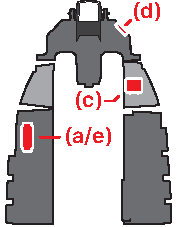
\includegraphics[
            width = \cockpitfigwidth,
        ]{F16_proc_start-up_engine-start_v01.pdf}
        \captionof{figure}{\textbf{Engine Start}}
    }
    \begin{subenumerate}
        \item \textbf{JFS Switch} \dotfill \textbf{START 2}
        \item \textbf{Throttle} \dotfill \textbf{IDLE} \\
        \hfill (\emph{once 20\% RPM reached})
        \item \textbf{SEC Light} \dotfill \textbf{OFF} 
        \item \textbf{ENGINE Warning Light} \dotfill \textbf{OFF} \\
        \hfill (\emph{once 60\% RPM reached})
        \item \textbf{JFS Switch} \dotfill \textbf{Confirm OFF}
    \end{subenumerate}\cbend}
    \blueitem{ENG Instruments}{
    \marginpar{%
        \centering
        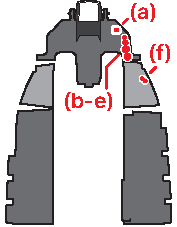
\includegraphics[
            width = \cockpitfigwidth,
        ]{F16_proc_start-up_engine-instruments_v01.pdf}
        \captionof{figure}{\textbf{ENG Instruments}}
    }
    \begin{subenumerate}
        \item \textbf{FUEL FLOW} -- 700-1700 PPH
        \item \textbf{OIL Pressure} -- 15 PSI (minimum)
        \item \textbf{NOZ POS} -- greater than 95\%
        \item \textbf{RPM} -- 62-80\% 
        \item \textbf{FTIT} -- 650C or less
        \item \textbf{HYD PRES A \& B} -- 2850-3250 PSI
    \end{subenumerate}}
\end{checklistenumerate}

\notebox{
    \begin{itemize}
        \item \textbf{Can close Canopy prior to advancing Throttle to IDLE to reduce cockpit noise}
    \end{itemize}
}

\clearpage

\subsection{POST-START}
\begin{checklistenumerate}
    \blueitem{TEST Panel}{
    \marginpar{%
        \centering
        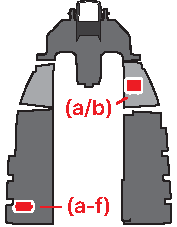
\includegraphics[
            width = \cockpitfigwidth,
        ]{F16_proc_start-up_test-panel_v01.pdf}
        \captionof*{figure}{\textbf{1. TEST Panel}}
    }
    \begin{subenumerate}
        \item \textbf{PROBE HEAT Switch} \dotfill \textbf{PROBE HEAT} \\
        \hfill \emph{verify PROBE HEAT Caution Light -- off}
        \item \textbf{PROBE HEAT Switch} \dotfill \textbf{TEST} \\
        \hfill \emph{verify PROBE HEAT Caution Light -- flashing}
        \item \textbf{PROBE HEAT Switch} \dotfill \textbf{OFF}
        \item \textbf{FIRE \& OHEAT DETECT} \dotfill \textbf{TEST}
        \item \textbf{OXY QTY Test Switch} \dotfill \textbf{TEST}
        \item \textbf{MAL \& IND LTS Button} \dotfill \textbf{TEST}
    \end{subenumerate}}
    \blueitem{AVIONICS Panel}{\cbstart
    \marginpar{%
        \centering
        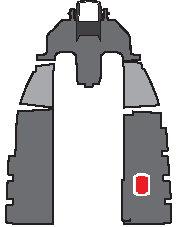
\includegraphics[
            width = \cockpitfigwidth,
        ]{F16_proc_start-up_avionics-ins_v01.pdf}
        \captionof*{figure}{\textbf{2./3. Avionics \& INS}}
    }
    \begin{subenumerate}
        \item \textbf{MMC Switch} \dotfill \textbf{MMC}
        \item \textbf{ST STA Switch} \dotfill \textbf{ST STA}
        \item \textbf{MFD Switch} \dotfill \textbf{MFD}
        \item \textbf{UFC Switch} \dotfill \textbf{UFD}
        \item \textbf{GPS Switch} \dotfill \textbf{GPS}
        \item \textbf{DL Switch} \dotfill \textbf{DL}
        \item \textbf{MIDS LVT Knob} \dotfill \textbf{ON}
    \end{subenumerate}}
    \blueitem{INS Alignment}{
    \begin{subenumerate}
        \item \textbf{EGI/INS} \dotfill \textbf{Desired ALIGN Mode} \\
        \begin{itemize}
            \item \textbf{NORM} -- Full alignment, approx. 8 min
            \item \textbf{STOR HDG} -- Quick alignment, approx. 90 sec
        \end{itemize}
    \end{subenumerate}}
    \blueitem{SNSR PWR Panel}{
    \marginpar{%
        \centering
        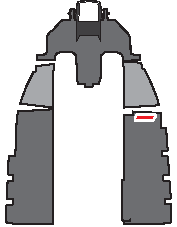
\includegraphics[
            width = \cockpitfigwidth,
        ]{F16_proc_start-up_snsr-pwr_v01.pdf}
        \captionof*{figure}{\textbf{4. SNSR PWR Panel}}
    }
    \begin{subenumerate}
        \item \textbf{LEFT HDPT Switch} \dotfill \textbf{As Required} \\
        \hfill \emph{if HTS Pod installed}
        \item \textbf{RIGHT HDPT Switch} \dotfill \textbf{As Required} \\
        \hfill \emph{if Targetting Pod installed}
        \item \textbf{FCR Switch} \dotfill \textbf{FCR}
        \item \textbf{RDR ALT Switch} \dotfill \textbf{RDR ALT}
    \end{subenumerate}\cbend}
\end{checklistenumerate}

\clearpage

\begin{checklistenumerate}[resume]
    \blueitem{HUD Setup}{\cbstart
    \marginpar{%
        \centering
        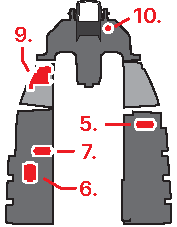
\includegraphics[
            width = \cockpitfigwidth,
        ]{F16_proc_start-up_hud-sai_v01.pdf}
        \captionof*{figure}{\textbf{5.-10. HUD, C\&I, ECM, SPD BRK, WHEELS Down, SAI}}
    }
    \begin{subenumerate}
        \item \textbf{HUD Control Panel} \dotfill \textbf{As Desired}
        \item \textbf{HUD Brightness} \dotfill \textbf{As Desired} 
    \end{subenumerate}\cbend}
    \blueitem{C\&I Knob}{\textbf{UFC}}
    \blueitem{ECM Panel}{\cbstart\textbf{As Desired}\cbend}
    \blueitem{SPD BRK Check}{\textbf{Cycle} (\emph{back to closed})}
    \blueitem{WHEELS Down Lights}{Verify \textbf{Three Green}}
    \blueitem{\cbstart  Standby Attitude Indicator\cbend}{\textbf{Set}}
    \blueitem{Tests \& Checks}{\hyperref[subsec:testschecks]{\textbf{See \Cref{subsec:testschecks} Tests \& Checks}}}
% \end{checklistenumerate}

% \clearpage

% \begin{checklistenumerate}[resume]
    \blueitem{Avionics Setup}{
    \marginpar{%
        \centering
        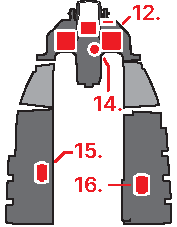
\includegraphics[
            width = \cockpitfigwidth,
        ]{F16_proc_start-up_final-setup_v01.pdf}
        \captionof*{figure}{\textbf{12.-16. Final Setup}}
    }
    \cbstart\textbf{Program As Required}}
    \blueitem{Canopy}{\textbf{Close and Lock}}
    \blueitem{Altimeter}{\textbf{Set and Check}}
    \blueitem{Exterior Lights}{\textbf{As Desired}}
    \blueitem{INS Knob}{\textbf{NAV}\cbend}
    \blueitem{NWS}{\textbf{Engage}}
    \blueitem{Throttle}{\textbf{Advance} (\emph{Check brakes \& NWS})}
    \blueitem{Flight Instruments}{\textbf{Check}}
\end{checklistenumerate}

% \clearpage

\warningbox{
    \begin{itemize}
        \item \textbf{Aircraft Rearming can interrupt INS align}
        \begin{itemize}
            \item If interrupted recycle INS knob to off, then back to align
            \item Recommend rearming either before or after INS align
        \end{itemize}
    \end{itemize}
}

\clearpage

\subsection{TESTS \& CHECKS}
\label{subsec:testschecks}
\begin{checklistenumerate}
    \blueitem{ENG SEC Mode}{
    \marginpar{%
        \centering
        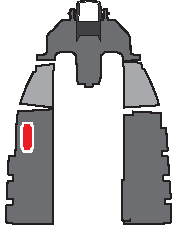
\includegraphics[
            width = \cockpitfigwidth,
        ]{F16_proc_start-up_check-eng-sec_v01.pdf}
        \captionof*{figure}{\textbf{1. ENG SEC Mode}}
    }
    \begin{subenumerate}
        \item \textbf{ENG CONT Switch} \dotfill \textbf{SEC}
        \begin{itemize}
            \item \textbf{SEC Caution Light} -- \textbf{ON}
            \item \textbf{RPM} -- Stabilized
            \item \textbf{Throttle} -- Snap to \textbf{MIL}, then to \textbf{IDLE} when RPM reaches 85\% 
            \item \textbf{NOZ POS} -- < 10\% within 30s after \textbf{SEC} selection
        \end{itemize}
        \item \textbf{ENG CONT Switch} \dotfill \textbf{PRI}
        \begin{itemize}
            \item \textbf{SEC Caution Light} -- \textbf{OFF}
            \item \textbf{NOZ POS} -- > 94\% 
        \end{itemize}
    \end{subenumerate}}
    \blueitem{FLCS BIT}{
    \marginpar{%
        \centering
        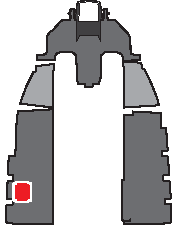
\includegraphics[
            width = \cockpitfigwidth,
        ]{F16_proc_start-up_check-flcs-bit_v01.pdf}
        \captionof*{figure}{\textbf{2. FLCS BIT}}
    }
    \begin{subenumerate}
        \item \textbf{FLCS BIT Switch} \dotfill \textbf{BIT}
        \begin{itemize}
            \item \textbf{FLCP RUN Light} -- Illuminates
        \end{itemize}
        \item \textbf{BIT Completion}
        \begin{itemize}
            \item \textbf{Duration} -- Approx. 45s
            \item \textbf{FLCP RUN Light} -- Extinguishes
            \item \textbf{BIT Switch} -- Returns to \textbf{OFF}
            \item \textbf{FAIL Light} -- Verify \textbf{OFF}
            \item \textbf{FLCS Warning Light} -- Verify \textbf{OFF}
        \end{itemize}
    \end{subenumerate}}
\end{checklistenumerate}

\clearpage

\begin{checklistenumerate}[resume]
    \blueitem{FUEL QTY Check}{
    \marginpar{%
        \centering
        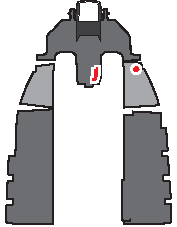
\includegraphics[
            width = \cockpitfigwidth,
        ]{F16_proc_start-up_check-fuel-qty_v01.pdf}
        \captionof*{figure}{\textbf{3. FUEL QTY Check}}
    }
    \begin{subenumerate}
        \item \textbf{FUEL QTY SEL Knob} \dotfill \textbf{TEST}
        \begin{itemize}
            \item \textbf{FR/AL Pointers} -- 2000 $\pm$ 100 lbs
            \item \textbf{Totalizer} -- 6000 $\pm$ 100 lbs
        \end{itemize}
        \item \textbf{FUEL QTY SEL Knob} \dotfill \textbf{NORM}
        \begin{itemize}
            \item \textbf{AL Pointer} -- 2675/2810 lbs
            \item \textbf{FR POINTER} -- 3100/3250 lbs
        \end{itemize}
        \item \textbf{FUEL QTY SEL Knob} \dotfill \textbf{RSVR}
        \begin{itemize}
            \item Each indicator approx. 460/480 lbs
        \end{itemize}
        \item \textbf{FUEL QTY SEL Knob} \dotfill \textbf{INT WING}
        \begin{itemize}
            \item Each indicator approx. 525/550 lbs
        \end{itemize}
        \item \textbf{FUEL QTY SEL Knob} \dotfill \textbf{EXT WING}
        \begin{itemize}
            \item Each indicator approx. 2300/2420 lbs
            \hfill (\emph{if loaded})
        \end{itemize}
        \item \textbf{FUEL QTY SEL Knob} \dotfill \textbf{As Desired}
    \end{subenumerate}}
    \blueitem{DBU Check}{
    \marginpar{%
        \centering
        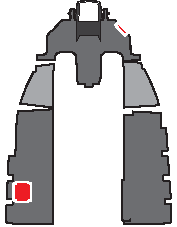
\includegraphics[
            width = \cockpitfigwidth,
        ]{F16_proc_start-up_check-dbu_v01.pdf}
        \captionof*{figure}{\textbf{4. DBU Check}}
    }
    \begin{subenumerate}
        \item \textbf{DIGITAL BACKUP Switch} \dotfill \textbf{BACKUP}
        \begin{itemize}
            \item \textbf{DBU ON Light} -- \textbf{Illuminates}
        \end{itemize}
        \item Operate Controls -- check for normal control surface response
        \item \textbf{DIGITAL BACKUP Switch} \dotfill \textbf{OFF}
    \end{subenumerate}}
    \blueitem{Trim Check}{
    \marginpar{%
        \centering
        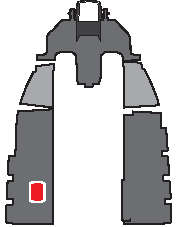
\includegraphics[
            width = \cockpitfigwidth,
        ]{F16_proc_start-up_check-trim_v01.pdf}
        \captionof*{figure}{\textbf{5. Trim Check}}
    }
    \begin{subenumerate}
        \item \textbf{TRIM/AP DISC Swtich} \dotfill \textbf{DISC}
        \item \textbf{Stick Trim} \dotfill Activate in Pitch \& Roll
        \begin{itemize}
            \item No control surface motion 
            \item No TRIM wheel or indicator motion
        \end{itemize} 
        \item \textbf{TRIM/AP DISC Swtich} \dotfill \textbf{NORM}
        \item \textbf{Stick Trim} \dotfill Check \& Center
        \begin{itemize}
            \item Control surface motion 
            \item TRIM wheel motion
        \end{itemize} 
        \item \textbf{Yaw Trim Knob} \dotfill \textbf{Center}
    \end{subenumerate}}
\end{checklistenumerate}

\clearpage

\begin{checklistenumerate}[resume]
    \blueitem{MPO Check}{
    \marginpar{%
        \centering
        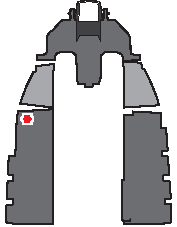
\includegraphics[
            width = \cockpitfigwidth,
        ]{F16_proc_start-up_check-mpo_v01.pdf}
        \captionof*{figure}{\textbf{6. MPO Check}}
    }
    \begin{subenumerate}
        \item \textbf{Stick} \dotfill \textbf{Full Forward \& Hold}
        \item \textbf{MPO Switch} \dotfill \textbf{OVRD \& Hold}
        \begin{itemize}
            \item Horizontal Tail trailing edges move farther down
        \end{itemize} 
        \item \textbf{Stick \& MPO} \dotfill Release
    \end{subenumerate}}
    \blueitem{EPU Check}{
    \marginpar
        \item \textbf{Throttle} \dotfill 10\% above \textbf{IDLE}
        \item \textbf{EPU/GEN TEST Switch} \dotfill \textbf{EPU/GEN \& Hold}
        \begin{itemize}
            \item \textbf{EPU AIR Light} -- \textbf{ON}
            \item \textbf{EPU GEN/PMG Lights} -- \textbf{OFF}
            \item \textbf{FLCS PWR Lights} -- \textbf{ON}
            \item \textbf{EPU Run Light} -- \textbf{ON} minimum 5s
        \end{itemize} 
        \item \textbf{EPU/GEN TEST Switch} \dotfill \textbf{OFF}
        \item \textbf{Throttle} \dotfill \textbf{IDLE}
        \item \textbf{OXYGEN} \dotfill \textbf{NORMAL}
    \end{subenumerate}}
\end{checklistenumerate}

\restoregeometry

\clearpage

\section{TAKEOFF \& LANDING}



\cleardoublepage